\documentclass[10pt]{article}

% Include Theme
% Margins ----------------------------------------------------------------------

\usepackage[margin=1.25in]{geometry}

% AMS --------------------------------------------------------------------------

\usepackage{amsmath}
\usepackage{amsfonts}
\usepackage{amsthm}
\usepackage{graphicx}


% Line Spacing -----------------------------------------------------------------

\renewcommand{\baselinestretch}{1.5}


% Font -------------------------------------------------------------------------

\usepackage[T1]{fontenc}
\usepackage[default]{lato}
% \usepackage[utopia, varg]{newtxmath}
% \renewcommand{\rmdefault}{futs} % Utopia as text font 

% Small adjustments to text kerning
\usepackage{microtype}

% Remove annoying over-full box warnings
\vfuzz2pt 
\hfuzz2pt


% Tikz support -----------------------------------------------------------------

\usepackage{tikz}


% Color Palette ----------------------------------------------------------------

\usepackage{xcolor}

% https://www.materialpalette.com/colors
\definecolor{dark-maroon}{HTML}{5D0F0D}
\definecolor{navyblue}{HTML}{0A3044}

% https://www.viget.com/articles/color-contrast/
\definecolor{purple}{HTML}{5601A4}
\definecolor{navy}{HTML}{0D3D56}
\definecolor{ruby}{HTML}{9a2515}
\definecolor{alice}{HTML}{107895}
\definecolor{daisy}{HTML}{EBC944}
\definecolor{coral}{HTML}{F26D21}
\definecolor{kelly}{HTML}{829356}
\definecolor{cranberry}{HTML}{E64173}
\definecolor{jet}{HTML}{131516}
\definecolor{asher}{HTML}{555F61}
\definecolor{slate}{HTML}{314F4F}


% Hyperlinks -------------------------------------------------------------------

\usepackage{hyperref}
\hypersetup{
    colorlinks= true,
    citecolor= dark-maroon,
    linkcolor= dark-maroon,
    filecolor= dark-maroon,      
    urlcolor= dark-maroon,
}


% Citations --------------------------------------------------------------------

% note, natbib provides better hyperlinking
\usepackage{natbib}
\bibliographystyle{econ-aea}
% How to display multiple in \citet{}
\setcitestyle{comma,aysep={}}

% Define Theorems --------------------------------------------------------------

% Put proper spacing after Theorem #. 
\newtheoremstyle{spacing}
{}%          Space above, empty = `usual value'
{}%          Space below
% {\itshape}%  Body font
{}%  Body font
{}%          Indent amount (empty = no indent, \parindent = para indent)
{\bfseries\color{navyblue}}% Thm head font
{.\ }%         Punctuation after thm head
{2.5mm}%  Space after thm head: \newline = linebreak
{}%          Thm head spec

% note, theorem is the name that goes in \begin{} and Theorem is the name displayed as Theorem 1
\theoremstyle{spacing}
\newtheorem{theorem}{Theorem}
\newtheorem{proposition}{Proposition}
\newtheorem{assumption}{Assumption}
\newtheorem{remark}{Remark}
\newtheorem{example}{Example}


% Custom Math Definitions ------------------------------------------------------

\global\long\def\expec#1{\mathbb{E}\left[#1\right]}%
\newcommand{\condexpec}[2]{\mathbb{E}\left[#1 \ \vert \ #2\right]}
\global\long\def\prob#1{\mathbb{P}\left[#1\right]}%
\global\long\def\var#1{\mathrm{Var}\left[#1\right]}%
\global\long\def\cov#1{\mathrm{Cov}\left[#1\right]}%
\global\long\def\one{\mathbf{1}}%


% Titlepage --------------------------------------------------------------------

% \maketitle
\usepackage{titling}
\usepackage{setspace}

% title
\pretitle{\begin{spacing}{1}\begin{flushleft}\huge}
\posttitle{\end{flushleft}\end{spacing}\vspace{-5mm}}
% author, note don't use \and 
\preauthor{\begin{flushleft}\LARGE}
\postauthor{\end{flushleft}\vspace{-7.5mm}}
% date
\predate{\begin{flushleft}\Large\color{asher}}
\postdate{\end{flushleft}\vspace{-5mm}}

% Abstract
\renewenvironment{abstract}
 {\noindent\rule{\linewidth}{.5pt}\noindent}
 {\noindent\rule{\linewidth}{.5pt}}

% alternative abstract
% \renewenvironment{abstract}
% {
%   \centerline {\large \bfseries \scshape \color{navyblue} Abstract}
%   \begin{quote}
% }
% {\end{quote}}


% Section and Subsection Styling -----------------------------------------------

\usepackage[explicit]{titlesec}

\titleformat{\section}
  {\large \bf \color{navyblue}}
  {\thesection \,---}
  {0.25em}
  {#1}
  
\titleformat{\subsection}
  {\fontsize{11}{10}\it}
  {\thesubsection.}
  {1em}
  {#1}


% Footnote ---------------------------------------------------------------------

% Spacing between footnotes on same page
\addtolength{\footnotesep}{1mm}

% Space after footnote number
\let\oldfootnote\footnote
\renewcommand\footnote[1]{\oldfootnote{\ #1}}

% No footnote line
\renewcommand\footnoterule{}

% No supsercript in footer
\makeatletter
\renewcommand\@makefntext[1]{%
    \parindent 1em \noindent
    \hb@xt@1.8em{\hss\normalfont\@thefnmark.\hfill}#1
  }
\makeatother




% Enumerate/Itemize ------------------------------------------------------------

\usepackage{enumitem}
\setitemize{labelindent=0.5em,labelsep=0.25cm,leftmargin=*}
\setenumerate{labelindent=0.5em,labelsep=0.25cm,leftmargin=*}


% Table and Figure labelling ---------------------------------------------------

\usepackage{caption}

\DeclareCaptionLabelSeparator{threedash}{\,---\,}
\DeclareCaptionFont{navyblue}{\color{navyblue}}
\DeclareCaptionFont{jet}{\color{jet}}
\captionsetup[table]{format=plain, labelsep=threedash, font={navyblue, bf}}
\captionsetup[figure]{format=plain, labelsep=threedash, font={navyblue, bf}}

% Alternative: Left align captions
% \captionsetup[table]{labelfont=it, textfont={navyblue, bf}, labelsep=newline, justification=raggedright, singlelinecheck=off}
% \captionsetup[figure]{labelfont=it, textfont={navyblue, bf}, labelsep=newline, justification=raggedright, singlelinecheck=off}

% multifigure with \caption
% \begin{subfigure}\caption{} \end{subfigure}
\usepackage{subcaption}
\captionsetup[subfigure]{format=plain, font={jet, footnotesize, bf}}


% Tables -----------------------------------------------------------------------

% Fix \input with tables
% \input fails when \\ is at end of external .tex file
\makeatletter
\let\input\@@input
\makeatother

% Make tables/figures wider than \textwidth using:
% \begin{adjustbox}{width = 1.2\textwidth, center}
% \end{adjustbox}
\usepackage{adjustbox}

% Slighty more spacing between rows
\usepackage{array}
\renewcommand\arraystretch{1.25}

% Table with easy to use footnotes
% \begin{threeparttable}
%    \begin{tabular} ... \end{tabular}
%    \begin{tablenotes}
%        \item \textit{Notes.}
%    \end{tablenotes}  
% \end{threeparttable}
\usepackage[flushleft]{threeparttable}
\setlength\labelsep{0pt}

% \toprule, \cmidrule, \bottomrule
\usepackage{booktabs}

% If tables are too narrow, fill columns using:
% \begin{tabularx}{\linewidth}{cols}
% col-types: X - center, L - left, R -right
% If you want relative scale for columns: 
% >{\hsize=.8\hsize}X/L/R
\usepackage{tabularx}
\newcolumntype{L}{>{\raggedright\arraybackslash}X}
\newcolumntype{R}{>{\raggedleft\arraybackslash}X}
\newcolumntype{C}{>{\centering\arraybackslash}X}

% Landscape table 
% \begin{landscape} \pagestyle{lscaped} table... \end{landscsape}
% \usepackage{pdflscape} - rotates page left-side up in pdf
% \usepackage{lscape} - does not rotate page, only figure/table

\usepackage{pdflscape}

% For landscape, fix page number location
\usepackage{fancyhdr}
\fancypagestyle{lscaped}{%
    \fancyhf{}
    \renewcommand{\headrulewidth}{0pt}
    \textnormal
    \fancyfoot{%
        \tikz[remember picture,overlay]
        \node[outer sep=2.5cm,above,rotate=90] at (current page.east) {\thepage};
    }
}
  

% ------------------------------------------------------------------------------


% \maketitle info
\title{Difference-in-Differences with Geocoded Microdata}
\author{\href{https://kylebutts.com/}{Kyle Butts}\thanks{University of Colorado, Boulder. Email: \href{mailto:buttskyle96@gmail.com}{buttskyle96@gmail.com}.} % \ and Other Author}
}
\date{\today}

\newcommand{\dist}{\text{Dist}}

% pdf info
\hypersetup{pdftitle={Example Paper}, pdfauthor={Kyle Butts}}

\begin{document}

% Title Page -------------------------------------------------------------------
\maketitle

\begin{abstract}
    \dots

    \par~\par\noindent
    JEL-Classification: 
    \par\noindent
    Keywords: 
    \par
\end{abstract}
\newpage

% Paper ------------------------------------------------------------------------

% ------------------------------------------------------------------------------
\section{Introduction}
% ------------------------------------------------------------------------------

In recent years, there has a been a surge of precisely geocoded microdata that has allowed researchers to answer questions about the effects of `treatment' at a very granular level. When treatment is located at a specific point in space, a very common method of evaluating the effects of the treatment is to compare units within an inner-ring of a certain distance to the treatment with units just a bit futher in an outer-ring. This identification strategy is illustrated  in \autoref{fig:example-id}.

The appeal of this identification strategy, which I will label the `Ring method', is that under the assumption that unobservable variables change smoothly over space, then the counterfactual outcomes will approximately be equal between both rings.

% Figure: Example ID -----------------------------------------------------------

\begin{figure}[tb]
    \caption{Rings Method}
    \label{fig:example-id}

    \begin{adjustbox}{width = 0.4\textwidth, center}
        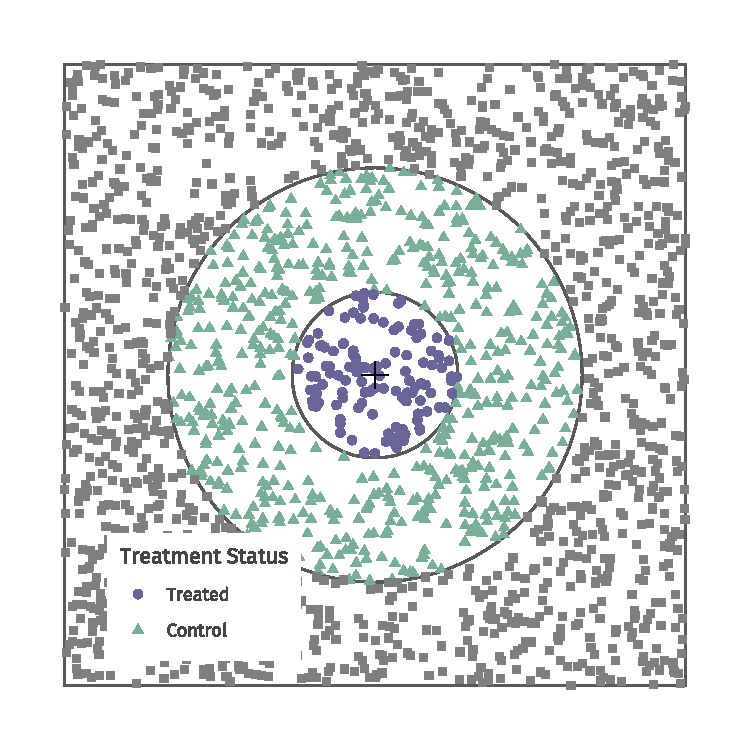
\includegraphics[width=\textwidth]{../figures/example_id.pdf}
    \end{adjustbox}
\end{figure}


% ------------------------------------------------------------------------------
\section{Example of Problem}
% ------------------------------------------------------------------------------

To illustrate the methodological difficulties in this method, I present an illustriative example. Suppose that an overgrown empty lot in a high-poverty neighborhood is cleaned up by the city and the outcome of interest is home prices. The researcher observes a panel of home sales before and after the lot is cleaned. Cleaning up the lot causes home values to go up directly nearby and as you move away from the lot, the positive treatment effect will decay to zero effect at, say, 3/4 of a mile.

% Figure: Example problem ------------------------------------------------------

\begin{figure}[tb]
    \caption{Example of Problems with Ad-Hoc Ring Selection}
    \label{fig:problems}
    
    \begin{adjustbox}{width = 1.1\textwidth, center}
        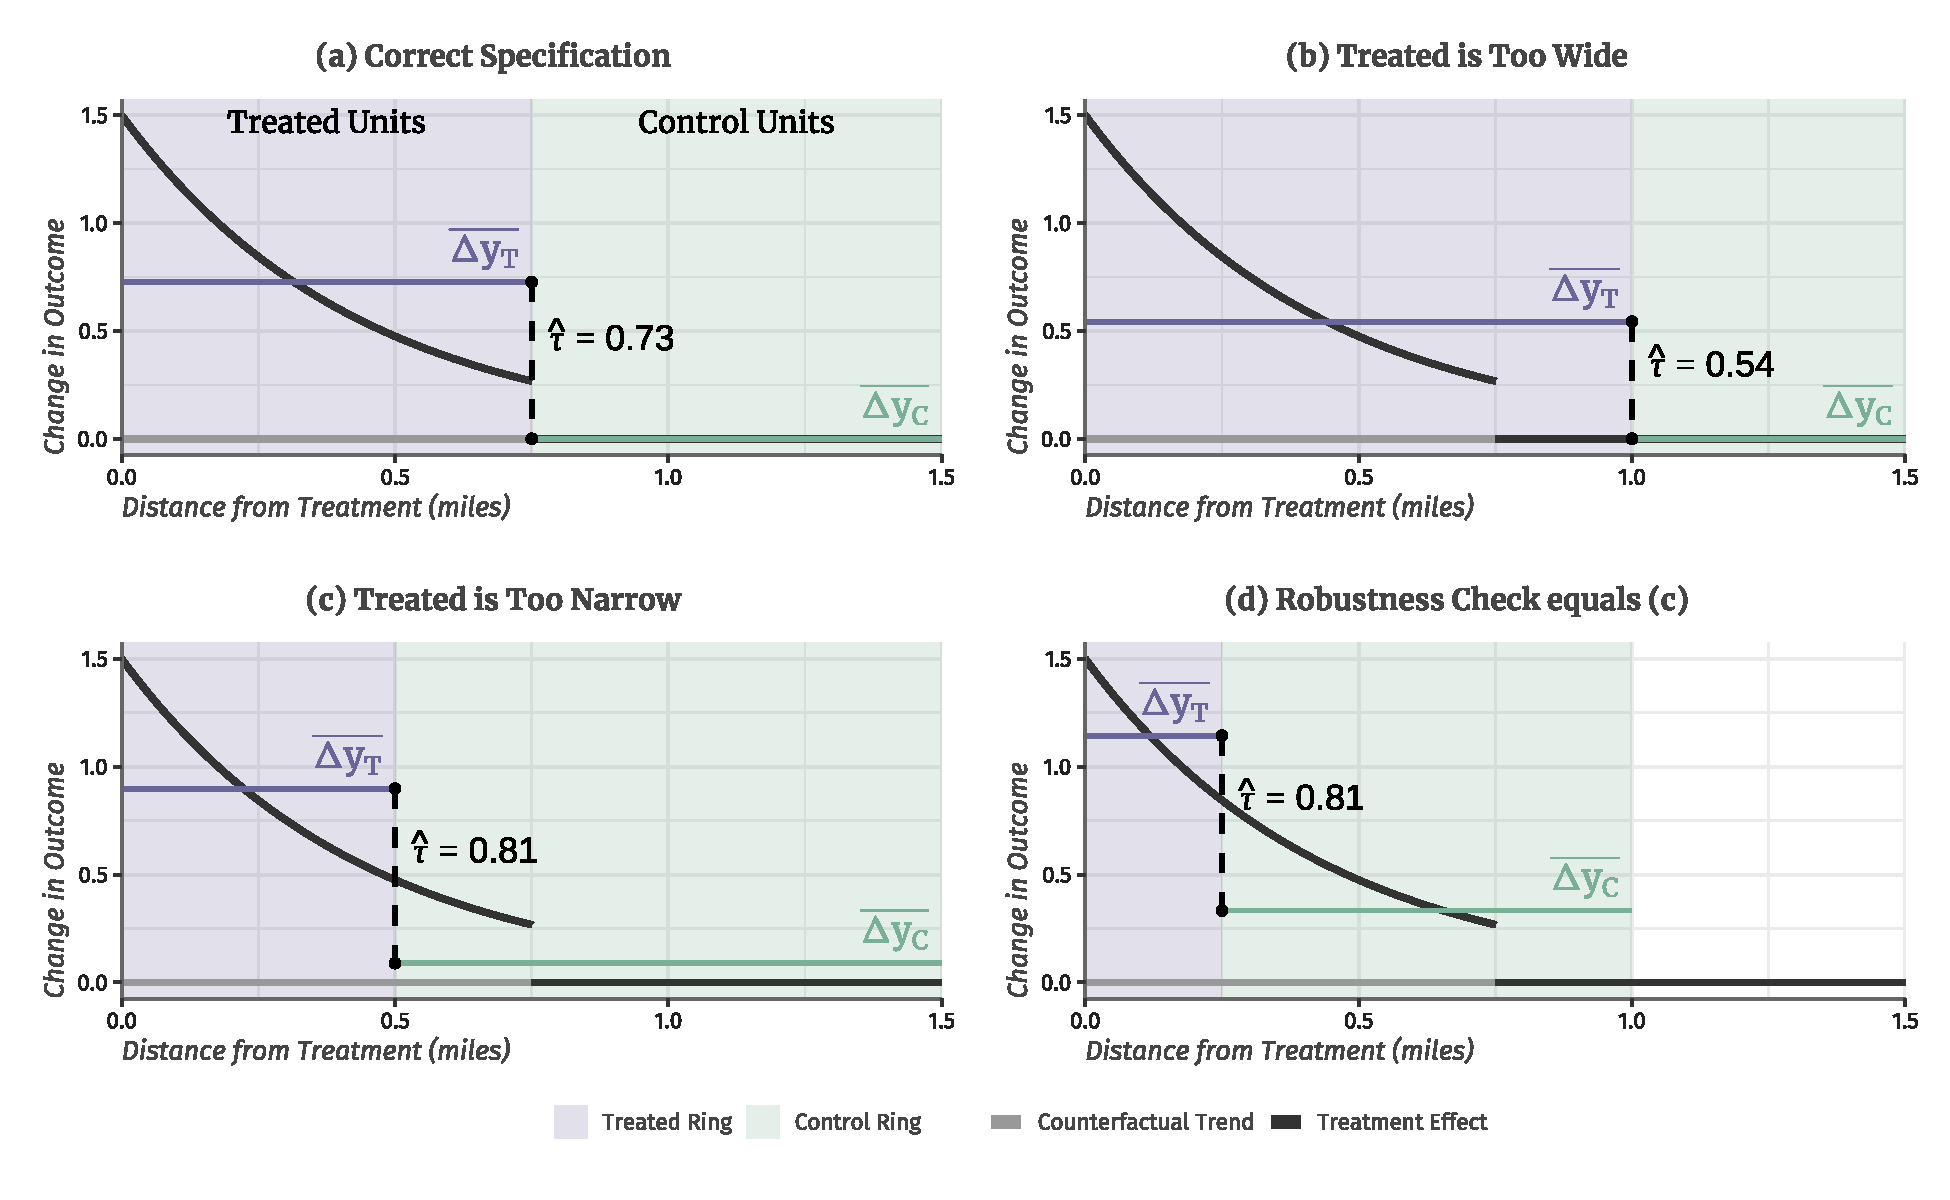
\includegraphics[width=\textwidth]{../figures/example.pdf}
    \end{adjustbox}
\end{figure}

\autoref{fig:problems} shows a plot of simulated data from this example. The black line is treatment effect at different distances from the empty lot and the grey line is the trend in home values at different distances from the empty lot. It is typically assumed that parallel trends hold at such a small radius from a location, so counterfactual trends are assumed to be constant in this example. Panel (a) of \autoref{fig:problems} shows the best-case scenario where the treated ring is correctly specified. The treatment effect estimate is the difference in the average change in outcome among the treated units and the control units. However, this singular number masks over a large amount of treatment effect heterogeneity with units very close to treatment having a treatment effect double that of $\hat{\tau}$ and units near 3/4 miles experience a treatment efffect half as large as $\hat{\tau}$. For this reason, even if a researcher identifies the correct average treatment effect, they are masking a lot of heterogeneity that is potentially interesting. Therefore, I recommend non-parametrically estimating the treatment effect as a function of distance rather than using a single indicator. 

However, the researcher does not typically know the distance at which treatment effects stop. Panels (b) and (c) highlights how treatment effect estimates change with a change in ring distances. Panel (b) shows when the `treatment' ring is too wide. In this case, some of the units in the treatment ring receive no effect from treatment and therefore makes the average treament effect among units in the treatment ring smaller. While this would be an accurate measure of the ``average'' treatment effect among the units in the treated ring, the estimated effect is not a measure of the average treatment effect among those actually affected by treatment that researchers aim to identify.

Panel (c) of \autoref{fig:problems} shows the opposite case, where the treated ring is too narrow. In this case, there are some units in the `control' ring that experience treatment effects. Hence, the average change in outcome among the control unit is too large. This does not, though, decrease the treatment effect as you may suspect. Since the treatment effect decays with distance, the average change in outcome among the more narrow ring is larger than the correct specification. The estimated treatment effect in this case grows. 

Often times, researchers try multiple sets of rings and if the estimated effect remains similar across specifications, they assume the results are `robust'. Panel (d) of \autoref{fig:problems} shows an example of why this a problem. If Panel (c) was the researchers' original specification and Panel (d) was run as a robustness check, then the researcher would be quite confident in their results even though the estimate is too large in both cases. 











% ------------------------------------------------------------------------------
\section{Theory}
% ------------------------------------------------------------------------------

A researcher observes panel data of units $i$ at times $t = 0, 1$ located in space at point $\theta_i = (x_i, y_i)$. Treatment occurs at a location $\bar{\theta} = (\bar{x}, \bar{y})$ between periods. Therefore, units differ in their distance to treatment, defined by $\dist_i \equiv \sqrt{(x_i - \bar{x})^2 + (y_i - \bar{y})^2}$. Since treatment location is often chosen strategically, potential outcomes will have to reflect the fact that trends can change with distance to treatment. Outcomes are given by 
\[ 
    Y_{it} = \tau(\dist_i) \one_{t = 1} + \mu_i + \lambda(\dist_i) \one_{t=1} + \varepsilon_{it},    
\]
where $\tau(\dist)$ is the treatment effect curve at different distances, $\mu_i$ is unit-specific time-invariant factors, and $\lambda(\dist)$ is the counterfactual trend at different distances from treatment. Since we include the $\lambda$ term, without loss of generality we assume that the error term $\varepsilon_{it}$ is uncorrelated with distance to treatment. Researchers are trying to identify the average treatment effect on units experiencing treatment effects, i.e. $\bar{\tau} = \condexpec{\tau(\dist)}{\tau(\dist) > 0}$ where expectations are with respect to the distribution of distances.

% \begin{assumption}[Random Sampling]
%     The observed data consists of $\{ Y_{i1}, Y_{i0}, \dist_{i}\}$ which is independent and identically distributed.
% \end{assumption}

Taking first differences, we see that $\Delta Y_{it} = \tau(\dist_i) + \lambda(\dist_i) + \Delta \varepsilon_{it}$. It is clear that $\tau(\dist_i)$ and $\lambda(\dist_i)$ are not seperately identified unless additional assumptions are imposed. Often times researchers claim that counterfactual trends likely evolve smoothly over distance, so that $\lambda(\dist_i)$ is approximately constant within a certain distance from treatment. This is formalized in the context of our outcome model by the following assumption. 

\begin{assumption}[Local Parallel Trends]\label{assum:parallel}
    For a distance $\bar{d}$, we say that local parallel trends hold if for all positive $d, d' \leq \bar{d}$, then $\lambda(d) = \lambda(d')$.
\end{assumption}

This assumption requires that, in the absence of treatment, outcomes would evolve the same at every distance from treatment within a certain maximum distance. The last assumption requires that researchers correctly specify $d_t$ to be the maximum distance that experience treatment effects. 

\begin{assumption}[Correct $d_t$]\label{assum:dt}
    A distance $d_t$ satisfies this assumption if for all $d \leq d_t$, $\tau(d) > 0$ and for all $d > d_t$, $\tau(d) = 0$. 
\end{assumption}


The `ring method' is the following procedure. Researchers select a pair of distances $d_t < d_c$ which define the ``treated'' and ``control'' groups. These groups are defined by $\mathcal{D}_t \equiv \{ i : 0 < \dist_i \leq d_t \}$ and $\mathcal{D}_c \equiv \{ i : d_t < \dist_i \leq d_c \}$. On the subsample of observations defined by $\mathcal{D} \equiv \mathcal{D}_t \cup \mathcal{D}_c$, they run the following specification:
\begin{equation}\label{eq:ring_method}
    \Delta Y_{it} = \beta_0 + \beta_1 \one_{i \in \mathcal{D}_t} + u_{it}.
\end{equation}

From our potential outcome framework and standard regression results, we have the following proposition.\footnote{A similar derivation is found in \citet{Sullivan_2017}.}

\begin{proposition}[Decomposition of Ring Estimate]\label{prop:ring_decomp}     
    \par~\par
    \begin{enumerate}
        \item[(i)] The estimate of $\beta_1$ in (\ref{eq:ring_method}) has the following expectation:
        \[
            \expec{\hat{\beta}_1} = 
            \underbrace{\condexpec{\tau(\dist)}{\mathcal{D}_t} - \condexpec{\tau(\dist)}{\mathcal{D}_c} }_{\text{Difference in Treatment Effect}} 
            + \underbrace{\condexpec{\lambda(\dist)}{\mathcal{D}_t} - \condexpec{\lambda(\dist)}{\mathcal{D}_c} }_{\text{Difference in Trends}}.
        \]
        
        \item[(ii)] More, if $d_c$ satisfies Assumption \ref{assum:parallel}, then
        \[ 
            \expec{\hat{\beta}_1} = 
            \underbrace{\condexpec{\tau(\dist)}{\mathcal{D}_t} - \condexpec{\tau(\dist)}{\mathcal{D}_c} }_{\text{Difference in Treatment Effect}}.
        \] 
    
        \item[(iii)] If $d_c$ satisfies Assumption \ref{assum:parallel} and $d_t$ satisfies Assumption \ref{assum:dt}, then
        \[ 
            \expec{\hat{\beta}_1} = \bar{\tau}.
        \]
    \end{enumerate}
    
    
\end{proposition}

This proposition shows that the `treatment effect' estimate is the sum of two differences. The first difference is the difference in average treatment effect among units in the treated ring and units in the control ring. If some units in the control group experience effects from treatment, the average of these effects will be subtracted from the estimate. The second difference is the difference in counterfactual trends between the treated and control rings. Since treatment can be targeted, the treated ring could be on a different trend than units further away. This difference in counterfactual trends is not seperately identifiable from the difference in average treatment effects unless Assumption \ref{assum:parallel} is satisfied. This is because if $d_c$ satisfies the assumption, then the counterfactual trend is absorbed completely by $\beta_0$ in Equation (\ref{eq:ring_method}).

As discussed above, the decomposition in part (ii) of Proposition \ref{prop:ring_decomp} is not necessarily unbiased estimate for $\bar{\tau}$. First, if $d_t$ is too wide, then $\mathcal{D}_t$ contain units that are not affected by treatment. In this case, first term will be smaller than $\bar{\tau}$ while the second term would be equal to zero since $d_c$ satisfies Assumption \ref{assum:parallel}. Therefore, $\hat{\beta}_1$ will be biased towards zero if $d_t$ is too wide. Second, if $d_t$ is too narrow then the $\mathcal{D}_c$ will contain units that experience treatment effects. It's not in this case, though, if $\hat{\beta_1}$ will grow or shrink without knowledge of the $\tau(\dist)$ curve. See the previous section for an example. 

The last result of Proposition \ref{prop:ring_decomp} shows that if $d_t$ is correctly specified as the maximum distance that receives treatment effect, then $\hat{\beta}_1$ will be an unbiased estimate for the average treatment effect among the untis affected by treatment. However, assumption \ref{assum:dt} is a very demanding assumption and unlikely to be known by the researcher. The following section will improve estimation by allowing non-parametric identification of $\tau(\dist)$. An estimate of $\tau(\dist)$ can then be numerically integrated to for an estimate of $\bar{\tau}$.










% ------------------------------------------------------------------------------
\newpage~\bibliography{references.bib}
% ------------------------------------------------------------------------------


\end{document}